\chapter{Les donn�es NMEA 0183}

%Ref : TV080114\_TU\_SM \hfill R�dacteur : Serge  Morvan \\



\section{Le standard NMEA}
http://standards.nmea.org/
Le site officiel : \\
 \hbox{}\hspace{1cm}\href{http://www.nmea.org/}{http://www.nmea.org/} \\
 Des informations sur le contenu des phrases : \\
 \hbox{}\hspace{1cm}\href{http://gpsinformation.net/}{http://gpsinformation.net/}\\
 \hbox{}\hspace{1cm}\href{http://gpsd.berlios.de/NMEA.html}{http://gpsd.berlios.de/NMEA.html}\\
 \hbox{}\hspace{1cm}\href{http://www.kh-gps.de/nmea.faq}{http://www.kh-gps.de/nmea.faq}\\
 Un projet de service d�mon :\\
 \hbox{}\hspace{1cm}\href{http://catb.org/gpsd/}{http://catb.org/gpsd/}\\

\newpage
\section{Mod�le NMEA0183}
\subsection{Ensemble des phrases analys�es}
\begin{center}
\framebox[1\width]{
	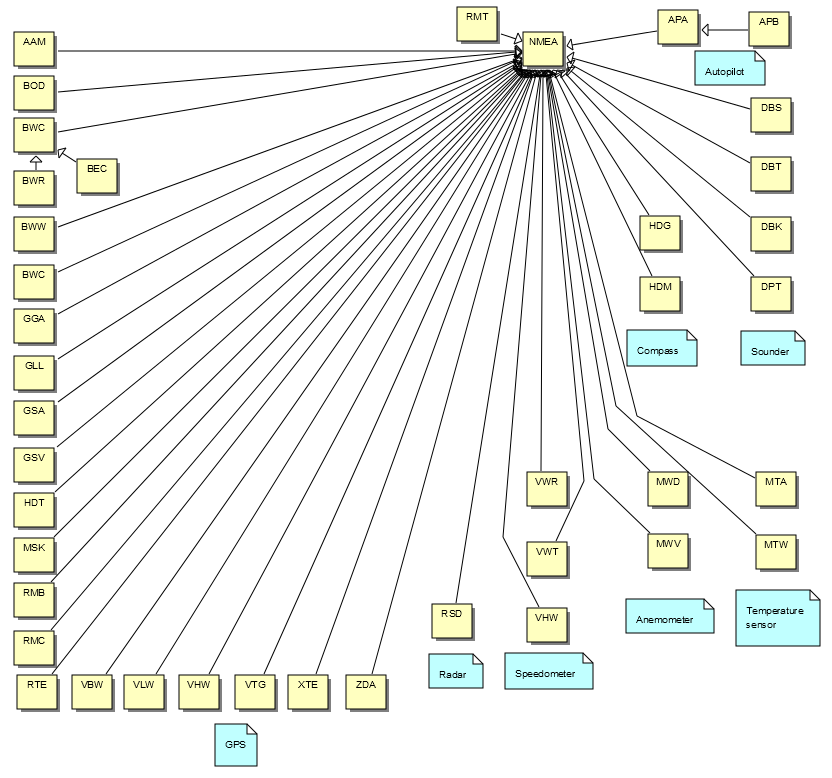
\includegraphics[width=18cm]{images/nmea/nmea.png}
}
\begin{figure}[h]
\caption{\label{nmea}\textit{Ensemble des classes de l'API NMEA}}
\end{figure}
\end{center}
%%%%%%%%%%%%%%%%%%%%%%%%%%%%%%%%%%%%%%%%%%%%%%%%%%%%%%%%%%%%%%%%%%%%%%%
%%%%%%%%%%%%%%%%%%%%%%%%%%%%%%%%%%%%%%%%%%%%%%%%%%%%%%%%%%%%%%%%%%%%%%
\begin{center}
\framebox[1\width]{
	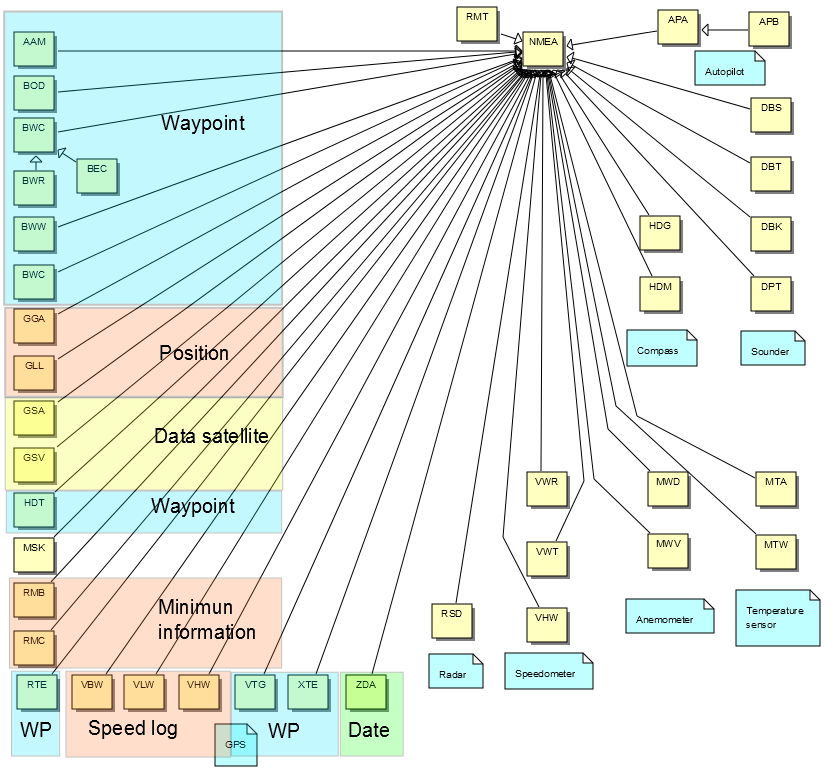
\includegraphics[width=17cm]{images/nmea/nmea_comment.png}
}
\begin{figure}[h]
\caption{\label{repart}\textit{Cat�gorisation des informations NMEA}}
\end{figure}
\end{center}
%%%%%%%%%%%%%%%%%%%%%%%%%%%%%%%%%%%%%%%%%%%%%%%%%%%%%%%%%%%%%%%%%%%%%%%
%%%%%%%%%%%%%%%%%%%%%%%%%%%%%%%%%%%%%%%%%%%%%%%%%%%%%%%%%%%%%%%%%%%%%%
\subsection{Minimun d'information pour la navigation}
\begin{center}
\framebox[1\width]{
	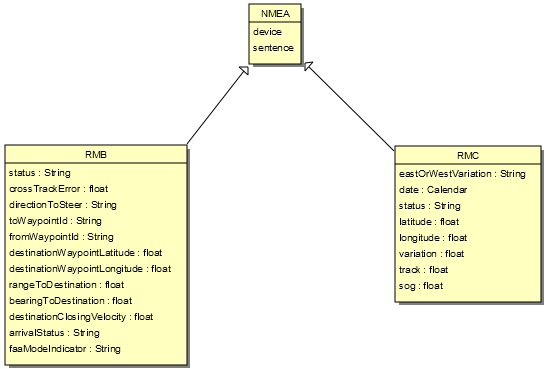
\includegraphics[width=16cm]{images/nmea/gps_minimum.png}
}
\begin{figure}[h]
\caption{\label{gpsminimum}\textit{Minimun d'information pour la navigation}}
\end{figure}
\end{center}
%%%%%%%%%%%%%%%%%%%%%%%%%%%%%%%%%%%%%%%%%%%%%%%%%%%%%%%%%%%%%%%%%%%%%%%
%%%%%%%%%%%%%%%%%%%%%%%%%%%%%%%%%%%%%%%%%%%%%%%%%%%%%%%%%%%%%%%%%%%%%%
\subsection{Date et heure}
\begin{center}
\framebox[1\width]{
	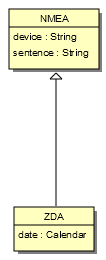
\includegraphics[width=3cm]{images/nmea/date.png}
}
\begin{figure}[h]
\caption{\label{date}\textit{Date}}
\end{figure}
\end{center}
%%%%%%%%%%%%%%%%%%%%%%%%%%%%%%%%%%%%%%%%%%%%%%%%%%%%%%%%%%%%%%%%%%%%%%%
%%%%%%%%%%%%%%%%%%%%%%%%%%%%%%%%%%%%%%%%%%%%%%%%%%%%%%%%%%%%%%%%%%%%%%
\subsection{Position : latitude, longitude}
\begin{center}
\framebox[1\width]{
	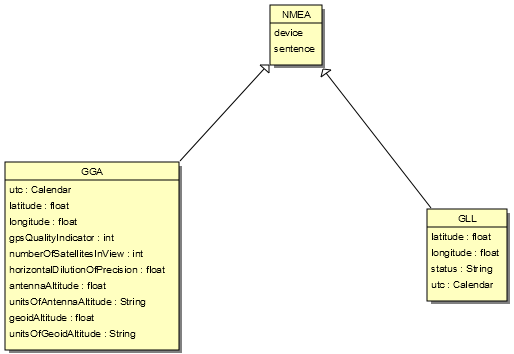
\includegraphics[width=16cm]{images/nmea/position.png}
}
\begin{figure}[h]
\caption{\label{position}\textit{Informations de position}}
\end{figure}
\end{center}
%%%%%%%%%%%%%%%%%%%%%%%%%%%%%%%%%%%%%%%%%%%%%%%%%%%%%%%%%%%%%%%%%%%%%%%
%%%%%%%%%%%%%%%%%%%%%%%%%%%%%%%%%%%%%%%%%%%%%%%%%%%%%%%%%%%%%%%%%%%%%%
\subsection{Informations de vitesse et de distance}
\begin{center}
\framebox[1\width]{
	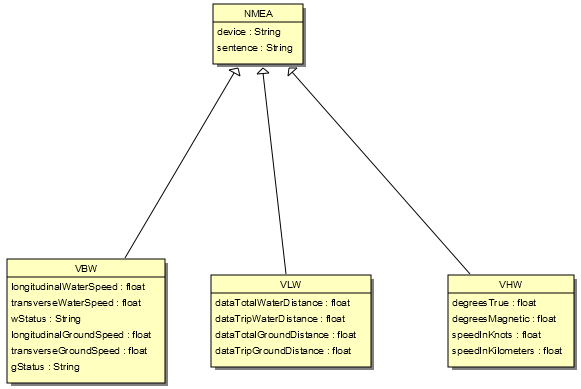
\includegraphics[width=16cm]{images/nmea/speedLog.png}
}
\begin{figure}[h]
\caption{\label{speedLog}\textit{Informations de vitesse et de distance}}
\end{figure}
\end{center}
%%%%%%%%%%%%%%%%%%%%%%%%%%%%%%%%%%%%%%%%%%%%%%%%%%%%%%%%%%%%%%%%%%%%%%%
%%%%%%%%%%%%%%%%%%%%%%%%%%%%%%%%%%%%%%%%%%%%%%%%%%%%%%%%%%%%%%%%%%%%%%
\subsection{Informations sur les waypoints}
\begin{center}
\framebox[1\width]{
	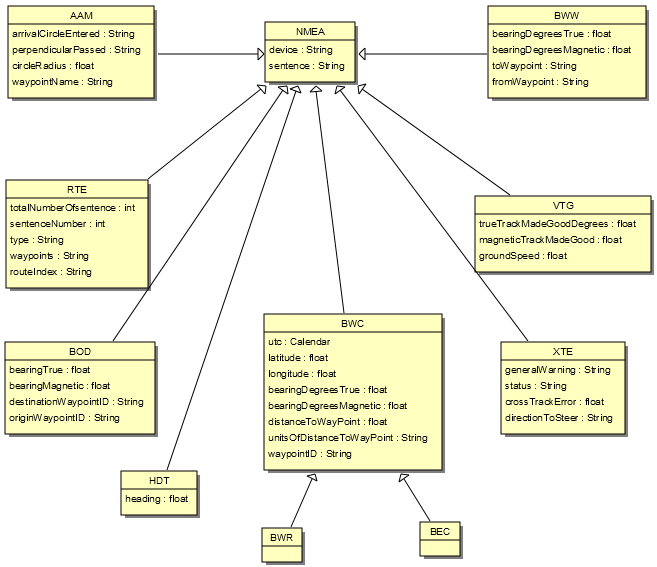
\includegraphics[width=16cm]{images/nmea/waypoint.png}
}
\begin{figure}[h]
\caption{\label{waypoint}\textit{Informations sur les waypoints}}
\end{figure}
\end{center}
%%%%%%%%%%%%%%%%%%%%%%%%%%%%%%%%%%%%%%%%%%%%%%%%%%%%%%%%%%%%%%%%%%%%%%%
%%%%%%%%%%%%%%%%%%%%%%%%%%%%%%%%%%%%%%%%%%%%%%%%%%%%%%%%%%%%%%%%%%%%%%
\subsection{Informations sur les satellites}
\begin{center}
\framebox[1\width]{
	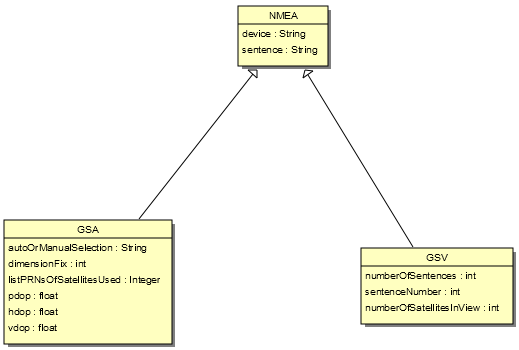
\includegraphics[width=16cm]{images/nmea/satellite.png}
}
\begin{figure}[h]
\caption{\label{satellite}\textit{Informations sur les satellites}}
\end{figure}
\end{center}

%%%%%%%%%%%%%%%%%%%%%%%%%%%%%%%%%%%%%%%%%%%%%%%%%%%%%%%%%%%%%%%%%%%%%%%
%%%%%%%%%%%%%%%%%%%%%%%%%%%%%%%%%%%%%%%%%%%%%%%%%%%%%%%%%%%%%%%%%%%%%%
\subsection{Informations sur le vent}
\begin{center}
\framebox[1\width]{
	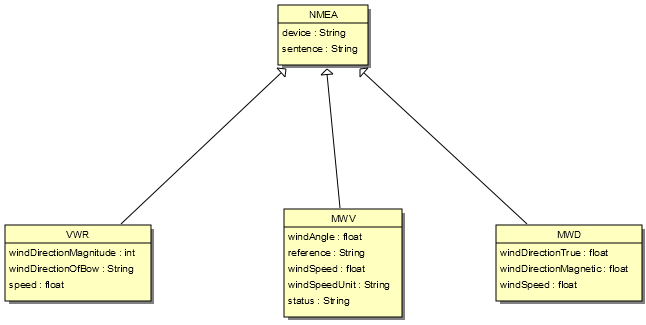
\includegraphics[width=16cm]{images/nmea/anemometer.png}
}
\begin{figure}[h]
\caption{\label{anemometer}\textit{Informations sur le vent}}
\end{figure}
\end{center}
%%%%%%%%%%%%%%%%%%%%%%%%%%%%%%%%%%%%%%%%%%%%%%%%%%%%%%%%%%%%%%%%%%%%%%%
%%%%%%%%%%%%%%%%%%%%%%%%%%%%%%%%%%%%%%%%%%%%%%%%%%%%%%%%%%%%%%%%%%%%%%
\subsection{Bathym�trie}
\begin{center}
\framebox[1\width]{
	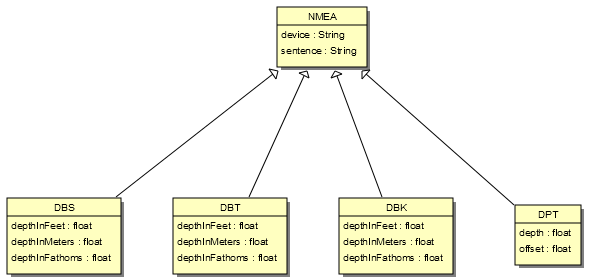
\includegraphics[width=16cm]{images/nmea/depth.png}
}
\begin{figure}[h]
\caption{\label{depth}\textit{Bathym�trie}}
\end{figure}
\end{center}
%%%%%%%%%%%%%%%%%%%%%%%%%%%%%%%%%%%%%%%%%%%%%%%%%%%%%%%%%%%%%%%%%%%%%%%

 %%%%%%%%%%%%%%%%%%%%%%%%%%%%%%%%%%%%%%%%%%%%%%%%%%%%%%%%%%%%%%%%%%%%%%
 \section{Pr�sentation de l'API}
 L'API permet l'acc�s au mod�le NMEA que nous avons choisit, celui-ci est proche
 de l'ensemble des phrases mais s'en �loigne parfois lorsqu'il y a redondance
 d'information dans une phrase, plusieurs valeurs de vitesse dans diff�rentes
 unit�s par exemple, ou lorsqu'une structure plus �labor�e permet de stocker des
 donn�es : liste, dictionnaire, \ldots
 \subsection{L'analyseur lexical et syntaxique}
 Le standard NMEA a beaucoup �volu�, plusieurs constructeurs ont impos� leur
 modifications, ce qui fait que de nombreuses variantes apparaissent dans les
 sorties NMEA des diff�rents appareils. Nous avons choisi d'uiliser le g�n�rateur
 d'analyseurs lexicaux et syntaxiques ANTLR pour plus de clart� du code. \\
 \hbox{}\hspace{1cm}\href{http://www.antlr.org/}{http://www.antlr.org/} \\
 \newpage
 En plus de cet outil nous utilisons l'atelier ANTLRWorks : \\ 
 \hbox{}\hspace{1cm}\href{http://www.antlr.org/works/}{http://www.antlr.org/works/}
 \\ Cet atelier permet de visualiser les grammaires cr��es.
 \subsubsection{Un exemple simple} 
 \small
 \begin{verbatim}
 GSV	     : '$' device=DEVICE 'GSV' 
 (NUMBER | SEP)+ 
 checksum=CHECKSUM
 { //action }
 \end{verbatim}
 \normalsize{}
 \begin{center}
 	\framebox[1\width]{
 		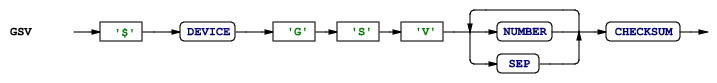
\includegraphics[width=12cm]{images/nmea/gsv.png}
 	}
 	\begin{figure}[h]
 		\caption{\label{gsv}\textit{Analyse de la phrase GSV}}
 	\end{figure}
 \end{center}
 
 \subsubsection{Un exemple plus complexe}
 \small
 \begin{verbatim}
 RMB     : '$' device = DEVICE 'RMB' SEP 
 status = LETTERS SEP  
 (crossTrackError =  NUMBER)* SEP
 (directionToSteer = LETTERS)* SEP
 (fromWaypointId = LETTERS |fromWaypointId = NUMBER)*  SEP
 (toWaypointId =  LETTERS | toWaypointId = NUMBER)* SEP
 (destinationWaypointLatitude =  NUMBER)* SEP (ns = LETTERS)* SEP
 (destinationWaypointLongitude  =  NUMBER)* SEP (ew  = LETTERS)* SEP
 (rangeToDestination =  NUMBER)* SEP
 (bearingToDestination =  NUMBER)* SEP
 (destinationClosingVelocity =  NUMBER)* SEP 	        	    
 (LETTERS SEP)*
 (arrivalStatus = LETTERS | '\u0000')* 
 checksum=CHECKSUM 
 { // action}
 \end{verbatim}
 \normalsize{}
 \begin{center}
 	\framebox[1\width]{
 		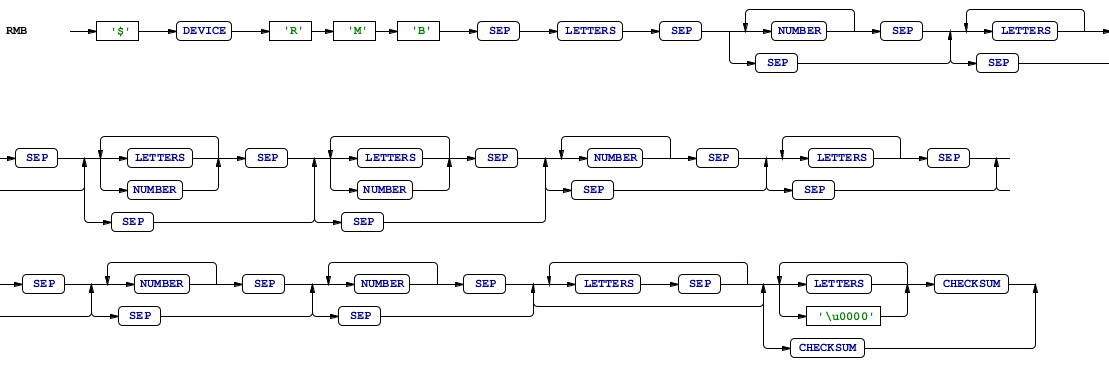
\includegraphics[width=12cm]{images/nmea/rmb.png}
 	}
 	\begin{figure}[h]
 		\caption{\label{dbt}\textit{Analyse de la phrase RMB}}
 	\end{figure}
 \end{center}
 
 %%%%%%%%%%%%%%%%%%%%%%%%%%%%%%%%%%%%%%%%%%%%%%%%%%%%%%%%%%%%%%%%%%%%%%

%%%%%%%%%%%%%%%%%%%%%%%%%%%%%%%%%%%%%%%%%%%%%%%%%%%%%%%%%%%%%%%%%%%%%%%

\section{Glossaire}
\begin{tabular}{|l|l|l|}
\hline
\bf Acronyme & \bf Expansion \\
\hline
AAM & Waypoint Arrival Alarm  \\
\hline
ALM & GPS Almanac Data \\
\hline
APA & Autopilot Sentence ``A''\\
\hline
APB  & Autopilot Sentence ``b''\\
\hline
BEC & Bearing and Distance to Waypoint,  Dead Reckoning\\
\hline
BOD & Bearing, Waypoint to Waypoint\\
\hline
BWC & Bearing and Distance to Waypoint\\
\hline
BWR  & Bearing and Distance to Waypoint   \\
\hline
BWW & Bearing and  Waypoint to Waypoint \\
\hline
DBK & Depth Below Keel \\
\hline
DBS & Depth Below Surface \\
\hline
DBT & Depth Below Transducer \\
\hline
DPT & Depth and offset \\
\hline
GGA &  Global Positioning System Fix Data. Time \\
\hline
GLL & Geographic Position and Latitude/Longitude \\
\hline
GSA & GPS DOP and active satellites \\
\hline
GSV & Satellites in view \\
\hline
GTD & Geographic Location in Time Differences \\
\hline
HDG & Heading, Deviation and Variation \\
\hline
HDM & Heading Magnetic \\
\hline
HDT & Heading True \\
\hline
MTW & Water Temperature \\
\hline
MWV & Wind Speed and Angle \\
\hline
RMA & Recommended Minimum Navigation Information \\
\hline
RMB & Recommended Minimum Navigation Information \\
\hline
RMC & Recommended Minimum Navigation Information \\
\hline
RTE & Routes \\
\hline
VBW & Dual Ground/Water Speed \\
\hline
VHW & Water Speed and Heading \\
\hline
VLW & Distance Traveled through Water \\
\hline
VPW & Speed, Measured Parallel to Wind \\
\hline
VTG & Track Made Good and Ground Speed \\
\hline
VWR & Relative Wind Speed and Angle \\
\hline
XTE & Cross-Track Error  Measured \\
\hline
ZDA & Time, Date and UTC, Day, Month, Year and Local Time Zone \\
\hline
\end{tabular}

